\lettrine[lines=3]{P}{}hysics simulations are becoming more common in many types of 3D graphics applications, particularly in video games. Physics engines such as Bullet, PhysX, Havok, and others are used to simulate anything from projectiles to ragdoll physics. These are known as physics engines because they are complex systems for simulating many common types of simulations. Simulating plant-life using a physics engine may be possible; however, these types of systems are continually being updated and changed. In order to keep this information relevant, this thesis will implement a full physics simulator to simulate plants generated by the L-system. Using a physics engine instead of the purpose-built simulator should be relatively straightforward, as the L-system generates a tree skeleton with all of the joint information such as width and length. Any other information that is needed can be provided through module parameters in the L-system and added to the joint information. Currently, the joint contains the following information: branch length, branch width, weight, spring constant, damping constant, momentum, as well as its rotation and position. 

This chapter will discuss a purpose-built method of simulating the physical motion of plant-life, laid out by Barron et al. \cite{barron2001real}. This method will be built so that it interacts with the L-system itself in such a way that the L-system can provide the parameters necessary for the simulation. This will allow a physics simulation to be run on any plant generated by the L-system.  

The primary technique discussed by Barron et al. for simulating the motion of a system like a tree or a plant, is taken from that of a particle system, first described by Reeves \cite{reeves1983particle}. Particle systems can be applied to simulate phenomena like clouds, smoke, water, and fire. The main advantage of particle systems is that the motion for each particle can be updated simultaneously. This technique can be applied to the L-system representation of plant-life, where branches are split into segments that make up a skeleton of segments or joints. Each joint can represent a \say{particle} within the system, which has a dependency on all of its parent branches.

The particle system concept can be used to simulate the motion of the plant by having each joint within the plant skeleton provide some basic physical properties. These properties include but are not limited to the width, length, direction vector, spring consistent, and dampening constant. The direction vector is the global direction that the branch is pointing in 3D space. The spring constant and the dampening constant are used in Hooke's Law calculations. The spring force of the branch resists it from bending. Whereas gravity, wind, and other forces generate torque, which generally acts against this spring force, causing the branch to bend.

\begin{figure}[htbp]
	{\centering
		\vspace{7px}
		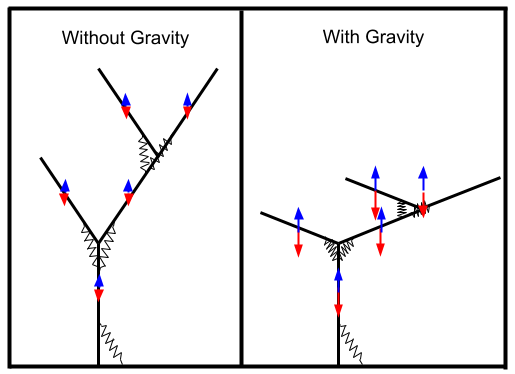
\includegraphics[scale=0.5]{Diagrams/HookesLaw.png}
		\caption{Diagram showing how Hooke's Law can be applied to a plant structure.} \label{rewriter diagram}
	}
\end{figure}
\FloatBarrier

This chapter defines a method of calculating the physical motion of a plant, where the properties can be defined in an L-system. The chapter starts by explaining how the volume, mass, inertia, and displacement of a given branch can be calculated. It then moves on to explain Hooke's Law and its role within the simulation of plant movement. The equations of motion in a 3D setting are then explained. Finally, this chapter talks about the challenges faced with efficiency when updating branches and some of the results that can be achieved by using this method. 

\section{Physical Properties of Branches}

The mass of each branch segment can be simply calculated by taking the volume of each branch and multiplying it by the density of the wood or material. To do this the volume of each branch needs to be calculated. This can be done by multiplying $\pi$ by the radius $r$ squared and the length $l$ as sees below.

\begin{equation}
v  = \pi r^2 l
\end{equation}

\noindent
The volume of the branch segment is not often a clean cylindrical shape, particularly if the branch segment is decreasing in size. However, it gives a good indication as to the volume of the branch. The volume can now be used to calculate the mass. Calculating the mass also requires the density of the material. For instance the density of pine wood is between 400 - 420 $\text{kg/m}^3$. Some woods being less dense at about 200 $\text{kg/m}^3$, and other hardwood being as dense as 1000$\text{kg/m}^3$. The denser the wood, the higher the mass, and ultimately the greater its resistance to its change in velocity.

\begin{equation}
m = v \times d
\end{equation}

\noindent
The mass can be used to calculate each branch segments' moment of inertia. The moment of inertia is the branches' resistance to angular momentum. As the object is 3D, the shape of the object needs to be taken into account. Each branch can be seen as a long cylinder, which can be expressed in the following equation.

\begin{equation}
I = \frac{1}{3} m l ^ 2
\end{equation}

\noindent
Where $I$ is the inertia of the branch, $m$ is the mass, and $l$ is the length. Similarly, an inertia tensor can be used for the sake of convenience to describe better the objects' rotational inertia, which is used within vector and matrix calculations. The inertia will be used when calculating the velocity of each segment in section \ref{motion equations}. Below is an inertia tensor for a shape that is similar to that of a branch segment.


\begin{equation}
\begin{aligned}
I = \begin{bmatrix}
\frac{1}{12}m(3r^2 + l^2) 	& 0 							& 0 \\
0 							& \frac{1}{12}m(3r^2 + l^2)		& 0 \\
0 							& 0 							& \frac{1}{2}mr^2 
\end{bmatrix}
\end{aligned}
\end{equation}

\noindent
The next vital piece of information needed is the direction that torque is acting on the branch ($V$), depending on the forces that are acting on it. The vector that represents the direction that the branch is pointing is known as the forward vector ($v$). The torque can be calculated by taking the cross product of the forward vector $v$ and the force vector $w$. This can be visualised using the right-hand rule, where the index finger is the forward vector, and the middle finger is the force vector. The direction of the thumb then points in the direction of the torque. The angular velocity is produced as spin in the direction around the torque vector.

\begin{equation}
V = v \otimes w
\end{equation}

\noindent
The displacement is the change of angle of a branch from its resting position and is used to calculate the spring force of the branch in Hooke's Law. The displacement can be calculated by keeping track of the starting local resting rotation of the branch $p$ as well as its current rotation $q$ in the form of two quaternions. The difference quaternion $d$ is calculated by taking the local resting rotation $p$ and multiplying it by the inverse of its current rotation $q$. 

\begin{equation}
d = p \times q^{-1}
\end{equation}

\section{Hooke's Law} \label{hookes law}

Hooke's law is a law of physics that states that the resultant force from compressing or extending a spring is equal to the product of the spring constant and the displacement of the spring. Each branch in a plant structure can be seen as a type of semi-rigid spring where external forces like gravity or wind bend the spring. Hooke's law is used to calculate the reaction force due to the displacement of the spring. Hooke's Law can be expressed in the equation below.

\begin{equation}
f = -k _s d + k _d v
\end{equation}

\noindent
Where $f$ is the force exerted by the spring, $k _s$ is the spring constant, and $d$ is the total displacement of the spring. The dampening force can be calculated as $k _d v$ part where $k _d$ is the dampening constant, and $v$ is the velocity at the end of the spring or branch.


\section{Equations of Motion} \label{motion equations}

All of the forces such as gravity, wind, and spring forces can then be multiplied together to get the net force $f_{net}$ acting on the spring. This is used to calculate the momentum of the branch, where $T_{delta}$ is the change in time between physics calculations.

\begin{equation}
M = M_0 + f_{net} * T_{delta}
\end{equation}

\noindent
The velocity $v$ is the current speed of the branch. In 3D graphics, the velocity is represented as a 3D vector and can be calculated by taking the inverse of the inertia tensor $I$ and multiplying that by the momentum vector $M$.

\begin{equation}
v = I^{-1} * M
Q_v = [0, v]
\end{equation}

\noindent
The velocity vector can be converted to its quaternion form $Q_v$ in order to make the last step simpler. The scalar part of a quaternion can be set to 0, and the vector part can be set to $v$. This allows the next rotation quaternion $R$ to be calculated. The last part involves taking the previous rotation quaternion, the velocity of the branch, and the change in time, to calculate the next quaternion rotation of the branch.

\begin{equation}
R = R_0 + (\frac{1}{2} * Q_v * R_0 * T_{delta})
\end{equation}

\noindent
$R$ is the next local rotation quaternion, $R_0$ is the previous local rotation quaternion, $Q_v$ is the velocity quaternion, and finally, $T_{delta}$ is the change in time since the previous physics update. This new rotation quaternion can then replace the current local rotation of the branch, in turn, simulating the motion of the branch.

\section{Updating Branches}

The particles in this system are the joints within the trees' skeleton. All of the joints have to be updated in each update step. The updates can happen as frequently as needed. A consideration is that if the branches are not updated frequently enough, the animations will not look smooth. Effectively each update step needs to take the forces acting on each branch, its current position, and rotation and calculate the next position and rotation of that branch. This information is then used to generate the model of the tree once again. This position and rotation are passed to the renderer, which will render the result.

\newpage
\section{Summary}

This chapter outlined a method of simulating and animating a procedurally generated plant by representing each branch as a  particle in a larger particle system. The trees' skeleton provides the information about the location, rotation, dimensions, and properties of each branch. The skeleton is created during the interpretation stage, which is ultimately provided by the L-system. The properties of each branch can be simulated as a particle within the entire tree system. Due to the embarrassingly parallel nature of the system, each branch update can be computed in parallel, either on the \acrshort{cpu} or \acrshort{gpu}.    

